\documentclass[twoside]{book}

% Packages required by doxygen
\usepackage{fixltx2e}
\usepackage{calc}
\usepackage{doxygen}
\usepackage[export]{adjustbox} % also loads graphicx
\usepackage{graphicx}
\usepackage[utf8]{inputenc}
\usepackage{makeidx}
\usepackage{multicol}
\usepackage{multirow}
\PassOptionsToPackage{warn}{textcomp}
\usepackage{textcomp}
\usepackage[nointegrals]{wasysym}
\usepackage[table]{xcolor}

% Font selection
\usepackage[T1]{fontenc}
\usepackage[scaled=.90]{helvet}
\usepackage{courier}
\usepackage{amssymb}
\usepackage{sectsty}
\renewcommand{\familydefault}{\sfdefault}
\allsectionsfont{%
  \fontseries{bc}\selectfont%
  \color{darkgray}%
}
\renewcommand{\DoxyLabelFont}{%
  \fontseries{bc}\selectfont%
  \color{darkgray}%
}
\newcommand{\+}{\discretionary{\mbox{\scriptsize$\hookleftarrow$}}{}{}}

% Page & text layout
\usepackage{geometry}
\geometry{%
  a4paper,%
  top=2.5cm,%
  bottom=2.5cm,%
  left=2.5cm,%
  right=2.5cm%
}
\tolerance=750
\hfuzz=15pt
\hbadness=750
\setlength{\emergencystretch}{15pt}
\setlength{\parindent}{0cm}
\setlength{\parskip}{3ex plus 2ex minus 2ex}
\makeatletter
\renewcommand{\paragraph}{%
  \@startsection{paragraph}{4}{0ex}{-1.0ex}{1.0ex}{%
    \normalfont\normalsize\bfseries\SS@parafont%
  }%
}
\renewcommand{\subparagraph}{%
  \@startsection{subparagraph}{5}{0ex}{-1.0ex}{1.0ex}{%
    \normalfont\normalsize\bfseries\SS@subparafont%
  }%
}
\makeatother

% Headers & footers
\usepackage{fancyhdr}
\pagestyle{fancyplain}
\fancyhead[LE]{\fancyplain{}{\bfseries\thepage}}
\fancyhead[CE]{\fancyplain{}{}}
\fancyhead[RE]{\fancyplain{}{\bfseries\leftmark}}
\fancyhead[LO]{\fancyplain{}{\bfseries\rightmark}}
\fancyhead[CO]{\fancyplain{}{}}
\fancyhead[RO]{\fancyplain{}{\bfseries\thepage}}
\fancyfoot[LE]{\fancyplain{}{}}
\fancyfoot[CE]{\fancyplain{}{}}
\fancyfoot[RE]{\fancyplain{}{\bfseries\scriptsize Generated by Doxygen }}
\fancyfoot[LO]{\fancyplain{}{\bfseries\scriptsize Generated by Doxygen }}
\fancyfoot[CO]{\fancyplain{}{}}
\fancyfoot[RO]{\fancyplain{}{}}
\renewcommand{\footrulewidth}{0.4pt}
\renewcommand{\chaptermark}[1]{%
  \markboth{#1}{}%
}
\renewcommand{\sectionmark}[1]{%
  \markright{\thesection\ #1}%
}

% Indices & bibliography
\usepackage{natbib}
\usepackage[titles]{tocloft}
\setcounter{tocdepth}{3}
\setcounter{secnumdepth}{5}
\makeindex

% Hyperlinks (required, but should be loaded last)
\usepackage{ifpdf}
\ifpdf
  \usepackage[pdftex,pagebackref=true]{hyperref}
\else
  \usepackage[ps2pdf,pagebackref=true]{hyperref}
\fi
\hypersetup{%
  colorlinks=true,%
  linkcolor=blue,%
  citecolor=blue,%
  unicode%
}

% Custom commands
\newcommand{\clearemptydoublepage}{%
  \newpage{\pagestyle{empty}\cleardoublepage}%
}

\usepackage{caption}
\captionsetup{labelsep=space,justification=centering,font={bf},singlelinecheck=off,skip=4pt,position=top}

%===== C O N T E N T S =====

\begin{document}

% Titlepage & ToC
\hypersetup{pageanchor=false,
             bookmarksnumbered=true,
             pdfencoding=unicode
            }
\pagenumbering{alph}
\begin{titlepage}
\vspace*{7cm}
\begin{center}%
{\Large N3 Library }\\
\vspace*{1cm}
{\large Generated by Doxygen 1.8.14}\\
\end{center}
\end{titlepage}
\clearemptydoublepage
\pagenumbering{roman}
\tableofcontents
\clearemptydoublepage
\pagenumbering{arabic}
\hypersetup{pageanchor=true}

%--- Begin generated contents ---
\chapter{Data Structure Index}
\section{Data Structures}
Here are the data structures with brief descriptions\+:\begin{DoxyCompactList}
\item\contentsline{section}{\mbox{\hyperlink{struct____n3l__backward__data}{\+\_\+\+\_\+n3l\+\_\+backward\+\_\+data}} \\*Internal struct to share data between threads }{\pageref{struct____n3l__backward__data}}{}
\item\contentsline{section}{\mbox{\hyperlink{struct____n3l__forward__data}{\+\_\+\+\_\+n3l\+\_\+forward\+\_\+data}} \\*Internal struct to share data between threads }{\pageref{struct____n3l__forward__data}}{}
\item\contentsline{section}{\mbox{\hyperlink{struct__n3l__layer}{\+\_\+n3l\+\_\+layer}} }{\pageref{struct__n3l__layer}}{}
\item\contentsline{section}{\mbox{\hyperlink{struct__n3l__neuron}{\+\_\+n3l\+\_\+neuron}} }{\pageref{struct__n3l__neuron}}{}
\item\contentsline{section}{\mbox{\hyperlink{struct__n3l__weight}{\+\_\+n3l\+\_\+weight}} }{\pageref{struct__n3l__weight}}{}
\item\contentsline{section}{\mbox{\hyperlink{structN3LArgs}{N3\+L\+Args}} }{\pageref{structN3LArgs}}{}
\item\contentsline{section}{\mbox{\hyperlink{structN3LNetwork}{N3\+L\+Network}} }{\pageref{structN3LNetwork}}{}
\end{DoxyCompactList}

\chapter{File Index}
\section{File List}
Here is a list of all documented files with brief descriptions\+:\begin{DoxyCompactList}
\item\contentsline{section}{{\bfseries n3lib.\+h} }{\pageref{n3lib_8h}}{}
\item\contentsline{section}{src/\hyperlink{n3__act_8c}{n3\+\_\+act.\+c} \\*This file contains activation functions and their primitive }{\pageref{n3__act_8c}}{}
\item\contentsline{section}{src/{\bfseries n3\+\_\+act.\+h} }{\pageref{n3__act_8h}}{}
\item\contentsline{section}{src/\hyperlink{n3__backward_8c}{n3\+\_\+backward.\+c} \\*This file contains functions to backpropagate the error and adjusts the weights }{\pageref{n3__backward_8c}}{}
\item\contentsline{section}{src/{\bfseries n3\+\_\+backward.\+h} }{\pageref{n3__backward_8h}}{}
\item\contentsline{section}{src/\hyperlink{n3__file_8c}{n3\+\_\+file.\+c} \\*This file contains functions to import and save a network state }{\pageref{n3__file_8c}}{}
\item\contentsline{section}{src/{\bfseries n3\+\_\+file.\+h} }{\pageref{n3__file_8h}}{}
\item\contentsline{section}{src/\hyperlink{n3__forward_8c}{n3\+\_\+forward.\+c} \\*This file contains functions to forward the inputs provided to the outputs }{\pageref{n3__forward_8c}}{}
\item\contentsline{section}{src/{\bfseries n3\+\_\+forward.\+h} }{\pageref{n3__forward_8h}}{}
\item\contentsline{section}{src/\hyperlink{n3__header_8h}{n3\+\_\+header.\+h} \\*This file contains types, enums and structs definitions }{\pageref{n3__header_8h}}{}
\item\contentsline{section}{src/\hyperlink{n3__layer_8c}{n3\+\_\+layer.\+c} \\*This file contains functions to work with N3\+Layer type }{\pageref{n3__layer_8c}}{}
\item\contentsline{section}{src/{\bfseries n3\+\_\+layer.\+h} }{\pageref{n3__layer_8h}}{}
\item\contentsline{section}{src/\hyperlink{n3__misc_8c}{n3\+\_\+misc.\+c} \\*This file contains functions to simplify working with the library }{\pageref{n3__misc_8c}}{}
\item\contentsline{section}{src/{\bfseries n3\+\_\+misc.\+h} }{\pageref{n3__misc_8h}}{}
\item\contentsline{section}{src/\hyperlink{n3__network_8c}{n3\+\_\+network.\+c} \\*This file contains functions to work with \hyperlink{structN3LNetwork}{N3\+L\+Network} type }{\pageref{n3__network_8c}}{}
\item\contentsline{section}{src/{\bfseries n3\+\_\+network.\+h} }{\pageref{n3__network_8h}}{}
\item\contentsline{section}{src/\hyperlink{n3__neuron_8c}{n3\+\_\+neuron.\+c} \\*This file contains functions to work with N3\+L\+Neuron type }{\pageref{n3__neuron_8c}}{}
\item\contentsline{section}{src/{\bfseries n3\+\_\+neuron.\+h} }{\pageref{n3__neuron_8h}}{}
\end{DoxyCompactList}

\chapter{Data Structure Documentation}
\hypertarget{struct____n3l__backward__data}{}\section{\+\_\+\+\_\+n3l\+\_\+backward\+\_\+data Struct Reference}
\label{struct____n3l__backward__data}\index{\+\_\+\+\_\+n3l\+\_\+backward\+\_\+data@{\+\_\+\+\_\+n3l\+\_\+backward\+\_\+data}}


Internal struct to share data between threads.  




Collaboration diagram for \+\_\+\+\_\+n3l\+\_\+backward\+\_\+data\+:
\nopagebreak
\begin{figure}[H]
\begin{center}
\leavevmode
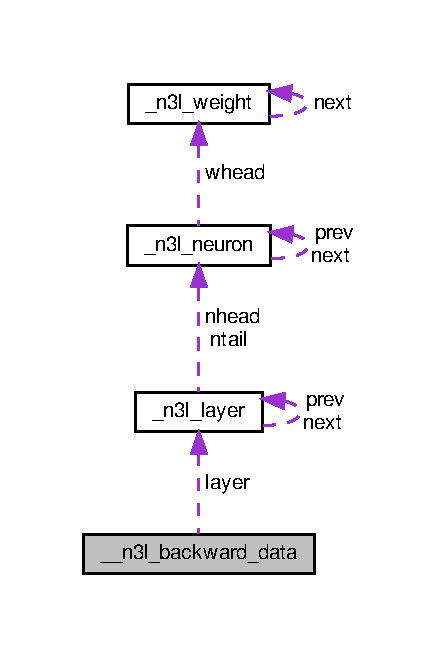
\includegraphics[width=210pt]{struct____n3l__backward__data__coll__graph}
\end{center}
\end{figure}
\subsection*{Data Fields}
\begin{DoxyCompactItemize}
\item 
uint64\+\_\+t \hyperlink{struct____n3l__backward__data_a32ef8a9b7e79121a563b8cd5486f88d3}{ref}
\item 
\hyperlink{n3__header_8h_a9ee3a7104816bdb6222148cfe9ca8ad9}{N3\+L\+Layer} $\ast$ \hyperlink{struct____n3l__backward__data_a0dcc17f32256df3e7ec65046236ffd24}{layer}
\item 
double \hyperlink{struct____n3l__backward__data_ab41bb2c143496d239fe41b208809cc85}{delta}
\item 
double \hyperlink{struct____n3l__backward__data_aa29c1bf7dcb85bfaaa0ec9b01cecc425}{learning\+\_\+rate}
\end{DoxyCompactItemize}


\subsection{Detailed Description}
Internal struct to share data between threads. 

Initialized from the current layer to the previous one. 

\subsection{Field Documentation}
\mbox{\Hypertarget{struct____n3l__backward__data_ab41bb2c143496d239fe41b208809cc85}\label{struct____n3l__backward__data_ab41bb2c143496d239fe41b208809cc85}} 
\index{\+\_\+\+\_\+n3l\+\_\+backward\+\_\+data@{\+\_\+\+\_\+n3l\+\_\+backward\+\_\+data}!delta@{delta}}
\index{delta@{delta}!\+\_\+\+\_\+n3l\+\_\+backward\+\_\+data@{\+\_\+\+\_\+n3l\+\_\+backward\+\_\+data}}
\subsubsection{\texorpdfstring{delta}{delta}}
{\footnotesize\ttfamily double \+\_\+\+\_\+n3l\+\_\+backward\+\_\+data\+::delta}

Delta evaluated \mbox{\Hypertarget{struct____n3l__backward__data_a0dcc17f32256df3e7ec65046236ffd24}\label{struct____n3l__backward__data_a0dcc17f32256df3e7ec65046236ffd24}} 
\index{\+\_\+\+\_\+n3l\+\_\+backward\+\_\+data@{\+\_\+\+\_\+n3l\+\_\+backward\+\_\+data}!layer@{layer}}
\index{layer@{layer}!\+\_\+\+\_\+n3l\+\_\+backward\+\_\+data@{\+\_\+\+\_\+n3l\+\_\+backward\+\_\+data}}
\subsubsection{\texorpdfstring{layer}{layer}}
{\footnotesize\ttfamily \hyperlink{n3__header_8h_a9ee3a7104816bdb6222148cfe9ca8ad9}{N3\+L\+Layer}$\ast$ \+\_\+\+\_\+n3l\+\_\+backward\+\_\+data\+::layer}

Previous layer \mbox{\Hypertarget{struct____n3l__backward__data_aa29c1bf7dcb85bfaaa0ec9b01cecc425}\label{struct____n3l__backward__data_aa29c1bf7dcb85bfaaa0ec9b01cecc425}} 
\index{\+\_\+\+\_\+n3l\+\_\+backward\+\_\+data@{\+\_\+\+\_\+n3l\+\_\+backward\+\_\+data}!learning\+\_\+rate@{learning\+\_\+rate}}
\index{learning\+\_\+rate@{learning\+\_\+rate}!\+\_\+\+\_\+n3l\+\_\+backward\+\_\+data@{\+\_\+\+\_\+n3l\+\_\+backward\+\_\+data}}
\subsubsection{\texorpdfstring{learning\+\_\+rate}{learning\_rate}}
{\footnotesize\ttfamily double \+\_\+\+\_\+n3l\+\_\+backward\+\_\+data\+::learning\+\_\+rate}

Learning rate set to the net \mbox{\Hypertarget{struct____n3l__backward__data_a32ef8a9b7e79121a563b8cd5486f88d3}\label{struct____n3l__backward__data_a32ef8a9b7e79121a563b8cd5486f88d3}} 
\index{\+\_\+\+\_\+n3l\+\_\+backward\+\_\+data@{\+\_\+\+\_\+n3l\+\_\+backward\+\_\+data}!ref@{ref}}
\index{ref@{ref}!\+\_\+\+\_\+n3l\+\_\+backward\+\_\+data@{\+\_\+\+\_\+n3l\+\_\+backward\+\_\+data}}
\subsubsection{\texorpdfstring{ref}{ref}}
{\footnotesize\ttfamily uint64\+\_\+t \+\_\+\+\_\+n3l\+\_\+backward\+\_\+data\+::ref}

Out neuron reference id 

The documentation for this struct was generated from the following file\+:\begin{DoxyCompactItemize}
\item 
src/\hyperlink{n3__backward_8c}{n3\+\_\+backward.\+c}\end{DoxyCompactItemize}

\hypertarget{struct____n3l__forward__data}{}\section{\+\_\+\+\_\+n3l\+\_\+forward\+\_\+data Struct Reference}
\label{struct____n3l__forward__data}\index{\+\_\+\+\_\+n3l\+\_\+forward\+\_\+data@{\+\_\+\+\_\+n3l\+\_\+forward\+\_\+data}}


Internal struct to share data between threads.  




Collaboration diagram for \+\_\+\+\_\+n3l\+\_\+forward\+\_\+data\+:
\nopagebreak
\begin{figure}[H]
\begin{center}
\leavevmode
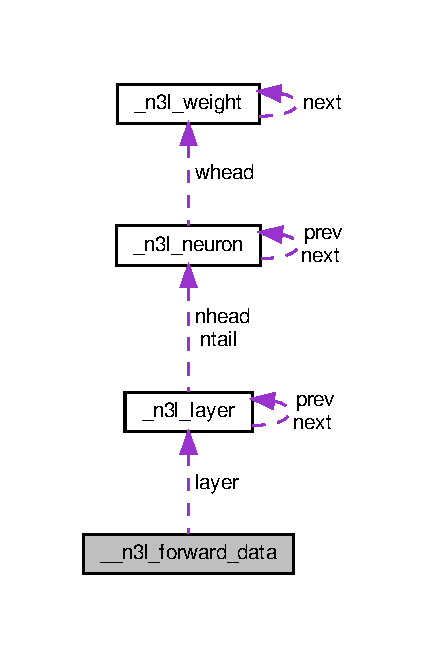
\includegraphics[width=205pt]{struct____n3l__forward__data__coll__graph}
\end{center}
\end{figure}
\subsection*{Data Fields}
\begin{DoxyCompactItemize}
\item 
uint64\+\_\+t \hyperlink{struct____n3l__forward__data_ada78b9bd1418f8dccab76319afb7d64b}{ref}
\item 
\hyperlink{n3__header_8h_a9ee3a7104816bdb6222148cfe9ca8ad9}{N3\+L\+Layer} $\ast$ \hyperlink{struct____n3l__forward__data_aaeb45910cc54c7f3a770dbd124477fc2}{layer}
\item 
double $\ast$ \hyperlink{struct____n3l__forward__data_ac870eae5ce14b297b5d78cc7112c8cec}{result}
\end{DoxyCompactItemize}


\subsection{Detailed Description}
Internal struct to share data between threads. 

Initialized from the current layer to the next one.

\begin{DoxySeeAlso}{See also}
\hyperlink{n3__forward_8c_ac55d957c2a3b754387f5037e87317870}{\+\_\+\+\_\+n3l\+\_\+forward\+\_\+get\+\_\+outputs} 
\end{DoxySeeAlso}


\subsection{Field Documentation}
\mbox{\Hypertarget{struct____n3l__forward__data_aaeb45910cc54c7f3a770dbd124477fc2}\label{struct____n3l__forward__data_aaeb45910cc54c7f3a770dbd124477fc2}} 
\index{\+\_\+\+\_\+n3l\+\_\+forward\+\_\+data@{\+\_\+\+\_\+n3l\+\_\+forward\+\_\+data}!layer@{layer}}
\index{layer@{layer}!\+\_\+\+\_\+n3l\+\_\+forward\+\_\+data@{\+\_\+\+\_\+n3l\+\_\+forward\+\_\+data}}
\subsubsection{\texorpdfstring{layer}{layer}}
{\footnotesize\ttfamily \hyperlink{n3__header_8h_a9ee3a7104816bdb6222148cfe9ca8ad9}{N3\+L\+Layer}$\ast$ \+\_\+\+\_\+n3l\+\_\+forward\+\_\+data\+::layer}

Current layer \mbox{\Hypertarget{struct____n3l__forward__data_ada78b9bd1418f8dccab76319afb7d64b}\label{struct____n3l__forward__data_ada78b9bd1418f8dccab76319afb7d64b}} 
\index{\+\_\+\+\_\+n3l\+\_\+forward\+\_\+data@{\+\_\+\+\_\+n3l\+\_\+forward\+\_\+data}!ref@{ref}}
\index{ref@{ref}!\+\_\+\+\_\+n3l\+\_\+forward\+\_\+data@{\+\_\+\+\_\+n3l\+\_\+forward\+\_\+data}}
\subsubsection{\texorpdfstring{ref}{ref}}
{\footnotesize\ttfamily uint64\+\_\+t \+\_\+\+\_\+n3l\+\_\+forward\+\_\+data\+::ref}

Next layer\textquotesingle{}s neuron reference \mbox{\Hypertarget{struct____n3l__forward__data_ac870eae5ce14b297b5d78cc7112c8cec}\label{struct____n3l__forward__data_ac870eae5ce14b297b5d78cc7112c8cec}} 
\index{\+\_\+\+\_\+n3l\+\_\+forward\+\_\+data@{\+\_\+\+\_\+n3l\+\_\+forward\+\_\+data}!result@{result}}
\index{result@{result}!\+\_\+\+\_\+n3l\+\_\+forward\+\_\+data@{\+\_\+\+\_\+n3l\+\_\+forward\+\_\+data}}
\subsubsection{\texorpdfstring{result}{result}}
{\footnotesize\ttfamily double$\ast$ \+\_\+\+\_\+n3l\+\_\+forward\+\_\+data\+::result}

Sum result while collecting outputs function 

The documentation for this struct was generated from the following file\+:\begin{DoxyCompactItemize}
\item 
src/\hyperlink{n3__forward_8c}{n3\+\_\+forward.\+c}\end{DoxyCompactItemize}

\hypertarget{struct__n3l__layer}{}\section{\+\_\+n3l\+\_\+layer Struct Reference}
\label{struct__n3l__layer}\index{\+\_\+n3l\+\_\+layer@{\+\_\+n3l\+\_\+layer}}


Double Linked List which contains layer\textquotesingle{}s values.  




{\ttfamily \#include $<$n3\+\_\+header.\+h$>$}



Collaboration diagram for \+\_\+n3l\+\_\+layer\+:\nopagebreak
\begin{figure}[H]
\begin{center}
\leavevmode
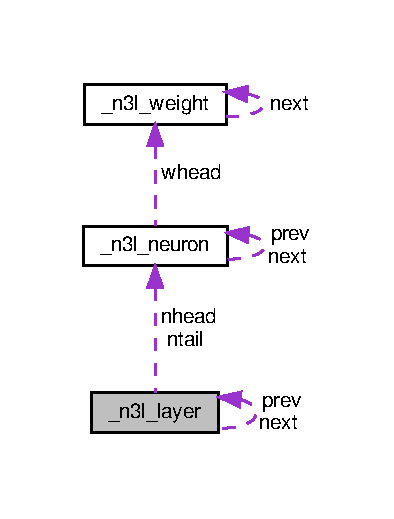
\includegraphics[width=189pt]{struct__n3l__layer__coll__graph}
\end{center}
\end{figure}
\subsection*{Data Fields}
\begin{DoxyCompactItemize}
\item 
\hyperlink{n3__header_8h_a1040baea07fec4d26d25641f75e892c5}{N3\+L\+Layer\+Type} \hyperlink{struct__n3l__layer_aec180f7f12ea86bb622c364076dbf1f6}{type}
\item 
\hyperlink{n3__header_8h_a621b1df037f351bd3542298933e5799a}{N3\+L\+Neuron} $\ast$ \hyperlink{struct__n3l__layer_a263e7831428a3b535964412a1d802c4e}{nhead}
\item 
\hyperlink{n3__header_8h_a621b1df037f351bd3542298933e5799a}{N3\+L\+Neuron} $\ast$ \hyperlink{struct__n3l__layer_aa120fe4ab0898e733b8d6940b467ebc3}{ntail}
\item 
struct \hyperlink{struct__n3l__layer}{\+\_\+n3l\+\_\+layer} $\ast$ \hyperlink{struct__n3l__layer_afada0fe8b2a403d5aeeb71b0ae7f8aae}{next}
\item 
struct \hyperlink{struct__n3l__layer}{\+\_\+n3l\+\_\+layer} $\ast$ \hyperlink{struct__n3l__layer_aedfd507c2c60e3b64234b8cd8570e6c9}{prev}
\end{DoxyCompactItemize}


\subsection{Detailed Description}
Double Linked List which contains layer\textquotesingle{}s values. 

The list is built by \hyperlink{n3__network_8c_a5f87e1efebd658dd55d7d2ca1768bdba}{n3l\+\_\+network\+\_\+build()} or \hyperlink{n3__file_8c_a4fef76548ed87845dceafaa9527a83d0}{n3l\+\_\+file\+\_\+import\+\_\+network()}.

\begin{DoxySeeAlso}{See also}
\hyperlink{struct__n3l__neuron}{\+\_\+n3l\+\_\+neuron}, \hyperlink{structN3LNetwork}{N3\+L\+Network}, \hyperlink{n3__layer_8c_a135215adb7cf8420293fd4ebd7049655}{n3l\+\_\+layer\+\_\+build}, \hyperlink{n3__layer_8c_ab06afb58d55be21a00bde5ee840f6425}{n3l\+\_\+layer\+\_\+count}, \hyperlink{n3__layer_8c_ad58e1630c1b7fc5da03d54cf63c394d9}{n3l\+\_\+layer\+\_\+free} 
\end{DoxySeeAlso}


\subsection{Field Documentation}
\mbox{\Hypertarget{struct__n3l__layer_afada0fe8b2a403d5aeeb71b0ae7f8aae}\label{struct__n3l__layer_afada0fe8b2a403d5aeeb71b0ae7f8aae}} 
\index{\+\_\+n3l\+\_\+layer@{\+\_\+n3l\+\_\+layer}!next@{next}}
\index{next@{next}!\+\_\+n3l\+\_\+layer@{\+\_\+n3l\+\_\+layer}}
\subsubsection{\texorpdfstring{next}{next}}
{\footnotesize\ttfamily struct \hyperlink{struct__n3l__layer}{\+\_\+n3l\+\_\+layer}$\ast$ \+\_\+n3l\+\_\+layer\+::next}

Next layer in the list or N\+U\+LL if it\textquotesingle{}s the last one. \mbox{\Hypertarget{struct__n3l__layer_a263e7831428a3b535964412a1d802c4e}\label{struct__n3l__layer_a263e7831428a3b535964412a1d802c4e}} 
\index{\+\_\+n3l\+\_\+layer@{\+\_\+n3l\+\_\+layer}!nhead@{nhead}}
\index{nhead@{nhead}!\+\_\+n3l\+\_\+layer@{\+\_\+n3l\+\_\+layer}}
\subsubsection{\texorpdfstring{nhead}{nhead}}
{\footnotesize\ttfamily \hyperlink{n3__header_8h_a621b1df037f351bd3542298933e5799a}{N3\+L\+Neuron}$\ast$ \+\_\+n3l\+\_\+layer\+::nhead}

Layer\textquotesingle{}s neuron list head. \begin{DoxySeeAlso}{See also}
\hyperlink{struct__n3l__neuron}{\+\_\+n3l\+\_\+neuron} 
\end{DoxySeeAlso}
\mbox{\Hypertarget{struct__n3l__layer_aa120fe4ab0898e733b8d6940b467ebc3}\label{struct__n3l__layer_aa120fe4ab0898e733b8d6940b467ebc3}} 
\index{\+\_\+n3l\+\_\+layer@{\+\_\+n3l\+\_\+layer}!ntail@{ntail}}
\index{ntail@{ntail}!\+\_\+n3l\+\_\+layer@{\+\_\+n3l\+\_\+layer}}
\subsubsection{\texorpdfstring{ntail}{ntail}}
{\footnotesize\ttfamily \hyperlink{n3__header_8h_a621b1df037f351bd3542298933e5799a}{N3\+L\+Neuron}$\ast$ \+\_\+n3l\+\_\+layer\+::ntail}

Layer\textquotesingle{}s neuron list tail. \begin{DoxySeeAlso}{See also}
\hyperlink{struct__n3l__neuron}{\+\_\+n3l\+\_\+neuron} 
\end{DoxySeeAlso}
\mbox{\Hypertarget{struct__n3l__layer_aedfd507c2c60e3b64234b8cd8570e6c9}\label{struct__n3l__layer_aedfd507c2c60e3b64234b8cd8570e6c9}} 
\index{\+\_\+n3l\+\_\+layer@{\+\_\+n3l\+\_\+layer}!prev@{prev}}
\index{prev@{prev}!\+\_\+n3l\+\_\+layer@{\+\_\+n3l\+\_\+layer}}
\subsubsection{\texorpdfstring{prev}{prev}}
{\footnotesize\ttfamily struct \hyperlink{struct__n3l__layer}{\+\_\+n3l\+\_\+layer}$\ast$ \+\_\+n3l\+\_\+layer\+::prev}

Previous layer in the list or N\+U\+LL if it\textquotesingle{}s the first one. \mbox{\Hypertarget{struct__n3l__layer_aec180f7f12ea86bb622c364076dbf1f6}\label{struct__n3l__layer_aec180f7f12ea86bb622c364076dbf1f6}} 
\index{\+\_\+n3l\+\_\+layer@{\+\_\+n3l\+\_\+layer}!type@{type}}
\index{type@{type}!\+\_\+n3l\+\_\+layer@{\+\_\+n3l\+\_\+layer}}
\subsubsection{\texorpdfstring{type}{type}}
{\footnotesize\ttfamily \hyperlink{n3__header_8h_a1040baea07fec4d26d25641f75e892c5}{N3\+L\+Layer\+Type} \+\_\+n3l\+\_\+layer\+::type}

Layer type. \begin{DoxySeeAlso}{See also}
\hyperlink{n3__header_8h_a1040baea07fec4d26d25641f75e892c5}{N3\+L\+Layer\+Type} 
\end{DoxySeeAlso}


The documentation for this struct was generated from the following file\+:\begin{DoxyCompactItemize}
\item 
src/\hyperlink{n3__header_8h}{n3\+\_\+header.\+h}\end{DoxyCompactItemize}

\hypertarget{struct__n3l__neuron}{}\section{\+\_\+n3l\+\_\+neuron Struct Reference}
\label{struct__n3l__neuron}\index{\+\_\+n3l\+\_\+neuron@{\+\_\+n3l\+\_\+neuron}}


Double Linked List which contains neuron\textquotesingle{}s values.  




{\ttfamily \#include $<$n3\+\_\+header.\+h$>$}



Collaboration diagram for \+\_\+n3l\+\_\+neuron\+:\nopagebreak
\begin{figure}[H]
\begin{center}
\leavevmode
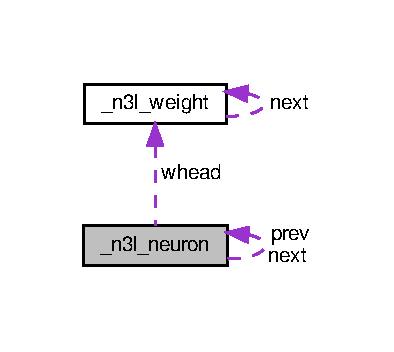
\includegraphics[width=189pt]{struct__n3l__neuron__coll__graph}
\end{center}
\end{figure}
\subsection*{Data Fields}
\begin{DoxyCompactItemize}
\item 
bool \hyperlink{struct__n3l__neuron_a0f3291ff81ab13111e538622ab662069}{bias}
\item 
uint64\+\_\+t \hyperlink{struct__n3l__neuron_aa0053e003b954df3b58853f003284958}{ref}
\item 
double \hyperlink{struct__n3l__neuron_ac896f5f8bd82c056cc61872120391048}{input}
\item 
\hyperlink{n3__header_8h_ac37c67a24ec253f5cd205cbc981922ca}{N3\+L\+Weight} $\ast$ \hyperlink{struct__n3l__neuron_ac9259a513822ea957c03430988adfa6a}{whead}
\item 
double \hyperlink{struct__n3l__neuron_afc9c38f4676dbe2ead749f8b6c81f491}{result}
\item 
\hyperlink{n3__header_8h_a3118e8995213ca26bd388c3d94cd8056}{N3\+L\+Act\+Type} \hyperlink{struct__n3l__neuron_af424e7accb8d1d089b828a1de69e03a0}{act\+\_\+type}
\item 
\hyperlink{n3__header_8h_afb10e6f7012513b51225a4d3add36cae}{N3\+L\+Act} \hyperlink{struct__n3l__neuron_a3ed17ddbe86d42ed6b7d31256b109262}{act}
\item 
\hyperlink{n3__header_8h_afb10e6f7012513b51225a4d3add36cae}{N3\+L\+Act} \hyperlink{struct__n3l__neuron_a9c9de65191cb097fd7a71752c83fc3db}{act\+\_\+prime}
\item 
struct \hyperlink{struct__n3l__neuron}{\+\_\+n3l\+\_\+neuron} $\ast$ \hyperlink{struct__n3l__neuron_a55f1bc3d589d69c5a940d0cb497610c4}{next}
\item 
struct \hyperlink{struct__n3l__neuron}{\+\_\+n3l\+\_\+neuron} $\ast$ \hyperlink{struct__n3l__neuron_a706ad4614fd4d1bd9a824f6ea8c0c9e5}{prev}
\end{DoxyCompactItemize}


\subsection{Detailed Description}
Double Linked List which contains neuron\textquotesingle{}s values. 

The list is built by n3l\+\_\+network\+\_\+build() or \hyperlink{n3__file_8c_a4fef76548ed87845dceafaa9527a83d0}{n3l\+\_\+file\+\_\+import\+\_\+network()}.

\begin{DoxySeeAlso}{See also}
\hyperlink{struct__n3l__layer}{\+\_\+n3l\+\_\+layer}, \hyperlink{struct__n3l__weight}{\+\_\+n3l\+\_\+weight}, n3l\+\_\+neuron\+\_\+build, n3l\+\_\+neuron\+\_\+count, n3l\+\_\+neuron\+\_\+free 
\end{DoxySeeAlso}


\subsection{Field Documentation}
\mbox{\Hypertarget{struct__n3l__neuron_a3ed17ddbe86d42ed6b7d31256b109262}\label{struct__n3l__neuron_a3ed17ddbe86d42ed6b7d31256b109262}} 
\index{\+\_\+n3l\+\_\+neuron@{\+\_\+n3l\+\_\+neuron}!act@{act}}
\index{act@{act}!\+\_\+n3l\+\_\+neuron@{\+\_\+n3l\+\_\+neuron}}
\subsubsection{\texorpdfstring{act}{act}}
{\footnotesize\ttfamily \hyperlink{n3__header_8h_afb10e6f7012513b51225a4d3add36cae}{N3\+L\+Act} \+\_\+n3l\+\_\+neuron\+::act}

Activation function. \begin{DoxySeeAlso}{See also}
\hyperlink{n3__header_8h_afb10e6f7012513b51225a4d3add36cae}{N3\+L\+Act} 
\end{DoxySeeAlso}
\mbox{\Hypertarget{struct__n3l__neuron_a9c9de65191cb097fd7a71752c83fc3db}\label{struct__n3l__neuron_a9c9de65191cb097fd7a71752c83fc3db}} 
\index{\+\_\+n3l\+\_\+neuron@{\+\_\+n3l\+\_\+neuron}!act\+\_\+prime@{act\+\_\+prime}}
\index{act\+\_\+prime@{act\+\_\+prime}!\+\_\+n3l\+\_\+neuron@{\+\_\+n3l\+\_\+neuron}}
\subsubsection{\texorpdfstring{act\+\_\+prime}{act\_prime}}
{\footnotesize\ttfamily \hyperlink{n3__header_8h_afb10e6f7012513b51225a4d3add36cae}{N3\+L\+Act} \+\_\+n3l\+\_\+neuron\+::act\+\_\+prime}

Activation function primitive. \begin{DoxySeeAlso}{See also}
\hyperlink{n3__header_8h_afb10e6f7012513b51225a4d3add36cae}{N3\+L\+Act} 
\end{DoxySeeAlso}
\mbox{\Hypertarget{struct__n3l__neuron_af424e7accb8d1d089b828a1de69e03a0}\label{struct__n3l__neuron_af424e7accb8d1d089b828a1de69e03a0}} 
\index{\+\_\+n3l\+\_\+neuron@{\+\_\+n3l\+\_\+neuron}!act\+\_\+type@{act\+\_\+type}}
\index{act\+\_\+type@{act\+\_\+type}!\+\_\+n3l\+\_\+neuron@{\+\_\+n3l\+\_\+neuron}}
\subsubsection{\texorpdfstring{act\+\_\+type}{act\_type}}
{\footnotesize\ttfamily \hyperlink{n3__header_8h_a3118e8995213ca26bd388c3d94cd8056}{N3\+L\+Act\+Type} \+\_\+n3l\+\_\+neuron\+::act\+\_\+type}

Activation function type. \begin{DoxySeeAlso}{See also}
\hyperlink{n3__header_8h_a3118e8995213ca26bd388c3d94cd8056}{N3\+L\+Act\+Type} 
\end{DoxySeeAlso}
\mbox{\Hypertarget{struct__n3l__neuron_a0f3291ff81ab13111e538622ab662069}\label{struct__n3l__neuron_a0f3291ff81ab13111e538622ab662069}} 
\index{\+\_\+n3l\+\_\+neuron@{\+\_\+n3l\+\_\+neuron}!bias@{bias}}
\index{bias@{bias}!\+\_\+n3l\+\_\+neuron@{\+\_\+n3l\+\_\+neuron}}
\subsubsection{\texorpdfstring{bias}{bias}}
{\footnotesize\ttfamily bool \+\_\+n3l\+\_\+neuron\+::bias}

Identifies if the neuron is a bias neuron. The bias neurons doesn\textquotesingle{}t get inputs and have N3\+L\+None as activation function. \begin{DoxyNote}{Note}
Usually there is only one bias neuron for each layer, except for the output one, and it\textquotesingle{}s built as last neuron.
\end{DoxyNote}
\begin{DoxySeeAlso}{See also}
\hyperlink{n3__act_8c_a8dc073371b15e2574897762b54f9326c}{n3l\+\_\+act\+\_\+none}, \hyperlink{structN3LArgs}{N3\+L\+Args}, n3l\+\_\+network\+\_\+build 
\end{DoxySeeAlso}
\mbox{\Hypertarget{struct__n3l__neuron_ac896f5f8bd82c056cc61872120391048}\label{struct__n3l__neuron_ac896f5f8bd82c056cc61872120391048}} 
\index{\+\_\+n3l\+\_\+neuron@{\+\_\+n3l\+\_\+neuron}!input@{input}}
\index{input@{input}!\+\_\+n3l\+\_\+neuron@{\+\_\+n3l\+\_\+neuron}}
\subsubsection{\texorpdfstring{input}{input}}
{\footnotesize\ttfamily double \+\_\+n3l\+\_\+neuron\+::input}

Neuron input value. This value is also used to apply activation fuction.

\begin{DoxySeeAlso}{See also}
\hyperlink{n3__forward_8c_a658e97e1260b05ef3d286fbe93f11a40}{\+\_\+\+\_\+n3l\+\_\+forward\+\_\+layer} 
\end{DoxySeeAlso}
\mbox{\Hypertarget{struct__n3l__neuron_a55f1bc3d589d69c5a940d0cb497610c4}\label{struct__n3l__neuron_a55f1bc3d589d69c5a940d0cb497610c4}} 
\index{\+\_\+n3l\+\_\+neuron@{\+\_\+n3l\+\_\+neuron}!next@{next}}
\index{next@{next}!\+\_\+n3l\+\_\+neuron@{\+\_\+n3l\+\_\+neuron}}
\subsubsection{\texorpdfstring{next}{next}}
{\footnotesize\ttfamily struct \hyperlink{struct__n3l__neuron}{\+\_\+n3l\+\_\+neuron}$\ast$ \+\_\+n3l\+\_\+neuron\+::next}

Next neuron in the list or N\+U\+LL if it\textquotesingle{}s the last one. \mbox{\Hypertarget{struct__n3l__neuron_a706ad4614fd4d1bd9a824f6ea8c0c9e5}\label{struct__n3l__neuron_a706ad4614fd4d1bd9a824f6ea8c0c9e5}} 
\index{\+\_\+n3l\+\_\+neuron@{\+\_\+n3l\+\_\+neuron}!prev@{prev}}
\index{prev@{prev}!\+\_\+n3l\+\_\+neuron@{\+\_\+n3l\+\_\+neuron}}
\subsubsection{\texorpdfstring{prev}{prev}}
{\footnotesize\ttfamily struct \hyperlink{struct__n3l__neuron}{\+\_\+n3l\+\_\+neuron}$\ast$ \+\_\+n3l\+\_\+neuron\+::prev}

Previous neuron in the list or N\+U\+LL if it\textquotesingle{}s the first one. \mbox{\Hypertarget{struct__n3l__neuron_aa0053e003b954df3b58853f003284958}\label{struct__n3l__neuron_aa0053e003b954df3b58853f003284958}} 
\index{\+\_\+n3l\+\_\+neuron@{\+\_\+n3l\+\_\+neuron}!ref@{ref}}
\index{ref@{ref}!\+\_\+n3l\+\_\+neuron@{\+\_\+n3l\+\_\+neuron}}
\subsubsection{\texorpdfstring{ref}{ref}}
{\footnotesize\ttfamily uint64\+\_\+t \+\_\+n3l\+\_\+neuron\+::ref}

Current neuron reference. \begin{DoxyWarning}{Warning}
This value must be unique into the network. It is used to collecting outputs in forward propagation and to evaluate delta in backward propagation.
\end{DoxyWarning}
\begin{DoxySeeAlso}{See also}
\hyperlink{n3__forward_8c_ac55d957c2a3b754387f5037e87317870}{\+\_\+\+\_\+n3l\+\_\+forward\+\_\+get\+\_\+outputs}, \hyperlink{n3__backward_8c_accf39951eeeca43985b286831dd397ce}{\+\_\+\+\_\+n3l\+\_\+backward\+\_\+execute} 
\end{DoxySeeAlso}
\mbox{\Hypertarget{struct__n3l__neuron_afc9c38f4676dbe2ead749f8b6c81f491}\label{struct__n3l__neuron_afc9c38f4676dbe2ead749f8b6c81f491}} 
\index{\+\_\+n3l\+\_\+neuron@{\+\_\+n3l\+\_\+neuron}!result@{result}}
\index{result@{result}!\+\_\+n3l\+\_\+neuron@{\+\_\+n3l\+\_\+neuron}}
\subsubsection{\texorpdfstring{result}{result}}
{\footnotesize\ttfamily double \+\_\+n3l\+\_\+neuron\+::result}

Neuron\textquotesingle{}s result. This value is initialiazed after forward propagation.

\begin{DoxySeeAlso}{See also}
\hyperlink{n3__forward_8c_abc37ac7f137db4d053e3b19ac8e6542a}{n3l\+\_\+forward\+\_\+propagation}, \hyperlink{n3__forward_8c_af014464aaf6842d7da0ee6d1b1570ffe}{\+\_\+\+\_\+n3l\+\_\+forward\+\_\+activate} 
\end{DoxySeeAlso}
\mbox{\Hypertarget{struct__n3l__neuron_ac9259a513822ea957c03430988adfa6a}\label{struct__n3l__neuron_ac9259a513822ea957c03430988adfa6a}} 
\index{\+\_\+n3l\+\_\+neuron@{\+\_\+n3l\+\_\+neuron}!whead@{whead}}
\index{whead@{whead}!\+\_\+n3l\+\_\+neuron@{\+\_\+n3l\+\_\+neuron}}
\subsubsection{\texorpdfstring{whead}{whead}}
{\footnotesize\ttfamily \hyperlink{n3__header_8h_ac37c67a24ec253f5cd205cbc981922ca}{N3\+L\+Weight}$\ast$ \+\_\+n3l\+\_\+neuron\+::whead}

Weight\textquotesingle{}s list head. \begin{DoxyNote}{Note}
It is set to N\+U\+LL if the neuron\textquotesingle{}s layer is of type N3\+L\+Output\+Layer
\end{DoxyNote}
\begin{DoxySeeAlso}{See also}
\hyperlink{struct__n3l__weight}{\+\_\+n3l\+\_\+weight}, \hyperlink{struct__n3l__layer}{\+\_\+n3l\+\_\+layer} 
\end{DoxySeeAlso}


The documentation for this struct was generated from the following file\+:\begin{DoxyCompactItemize}
\item 
src/\hyperlink{n3__header_8h}{n3\+\_\+header.\+h}\end{DoxyCompactItemize}

\hypertarget{struct__n3l__weight}{}\section{\+\_\+n3l\+\_\+weight Struct Reference}
\label{struct__n3l__weight}\index{\+\_\+n3l\+\_\+weight@{\+\_\+n3l\+\_\+weight}}


Collaboration diagram for \+\_\+n3l\+\_\+weight\+:\nopagebreak
\begin{figure}[H]
\begin{center}
\leavevmode
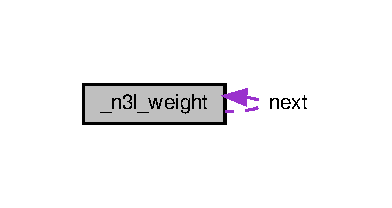
\includegraphics[width=188pt]{struct__n3l__weight__coll__graph}
\end{center}
\end{figure}
\subsection*{Data Fields}
\begin{DoxyCompactItemize}
\item 
\mbox{\Hypertarget{struct__n3l__weight_a1d1ebc5e04ba1dd26094993dd94aa710}\label{struct__n3l__weight_a1d1ebc5e04ba1dd26094993dd94aa710}} 
double {\bfseries value}
\item 
\mbox{\Hypertarget{struct__n3l__weight_ac5094b52f09a092ffb1cdc4cc594f38f}\label{struct__n3l__weight_ac5094b52f09a092ffb1cdc4cc594f38f}} 
uint64\+\_\+t {\bfseries target\+\_\+ref}
\item 
\mbox{\Hypertarget{struct__n3l__weight_adf96faae4820538377678c82ec96d48e}\label{struct__n3l__weight_adf96faae4820538377678c82ec96d48e}} 
struct \hyperlink{struct__n3l__weight}{\+\_\+n3l\+\_\+weight} $\ast$ {\bfseries next}
\end{DoxyCompactItemize}


The documentation for this struct was generated from the following file\+:\begin{DoxyCompactItemize}
\item 
src/n3\+\_\+header.\+h\end{DoxyCompactItemize}

\hypertarget{structN3LArgs}{}\section{N3\+L\+Args Struct Reference}
\label{structN3LArgs}\index{N3\+L\+Args@{N3\+L\+Args}}
\subsection*{Data Fields}
\begin{DoxyCompactItemize}
\item 
\mbox{\Hypertarget{structN3LArgs_ad51d108eba4b55f7fc49174724fbacad}\label{structN3LArgs_ad51d108eba4b55f7fc49174724fbacad}} 
double {\bfseries bias}
\item 
\mbox{\Hypertarget{structN3LArgs_afbd19ab7f7afe11e440f46d293a0f6dc}\label{structN3LArgs_afbd19ab7f7afe11e440f46d293a0f6dc}} 
uint64\+\_\+t {\bfseries in\+\_\+size}
\item 
\mbox{\Hypertarget{structN3LArgs_acbb947695cd6db88658a2a6fa78c1682}\label{structN3LArgs_acbb947695cd6db88658a2a6fa78c1682}} 
uint64\+\_\+t {\bfseries h\+\_\+layers}
\item 
\mbox{\Hypertarget{structN3LArgs_ae875ef755586a29387def48249c98d81}\label{structN3LArgs_ae875ef755586a29387def48249c98d81}} 
uint64\+\_\+t $\ast$ {\bfseries h\+\_\+size}
\item 
\mbox{\Hypertarget{structN3LArgs_a63bb20896b0af109ea281998e5fd56ab}\label{structN3LArgs_a63bb20896b0af109ea281998e5fd56ab}} 
uint64\+\_\+t {\bfseries out\+\_\+size}
\item 
\mbox{\Hypertarget{structN3LArgs_abb810a671b7a1b20c161e81e309f843c}\label{structN3LArgs_abb810a671b7a1b20c161e81e309f843c}} 
N3\+L\+Act\+Type {\bfseries act\+\_\+in}
\item 
\mbox{\Hypertarget{structN3LArgs_a968aa1ed194fc7bbfaac154bcbf8a405}\label{structN3LArgs_a968aa1ed194fc7bbfaac154bcbf8a405}} 
N3\+L\+Act\+Type $\ast$ {\bfseries act\+\_\+h}
\item 
\mbox{\Hypertarget{structN3LArgs_ad9d17026b32668acea535143809b16c5}\label{structN3LArgs_ad9d17026b32668acea535143809b16c5}} 
N3\+L\+Act\+Type {\bfseries act\+\_\+out}
\item 
\mbox{\Hypertarget{structN3LArgs_a9df79247b5160e5261683a535654cc18}\label{structN3LArgs_a9df79247b5160e5261683a535654cc18}} 
void $\ast$ {\bfseries rand\+\_\+arg}
\item 
\mbox{\Hypertarget{structN3LArgs_ac6f4a8939deb104e8b154860904f3b45}\label{structN3LArgs_ac6f4a8939deb104e8b154860904f3b45}} 
N3\+L\+Weight\+Generator {\bfseries rand\+\_\+weight}
\end{DoxyCompactItemize}


The documentation for this struct was generated from the following file\+:\begin{DoxyCompactItemize}
\item 
src/n3\+\_\+header.\+h\end{DoxyCompactItemize}

\hypertarget{structN3LNetwork}{}\section{N3\+L\+Network Struct Reference}
\label{structN3LNetwork}\index{N3\+L\+Network@{N3\+L\+Network}}


Collaboration diagram for N3\+L\+Network\+:\nopagebreak
\begin{figure}[H]
\begin{center}
\leavevmode
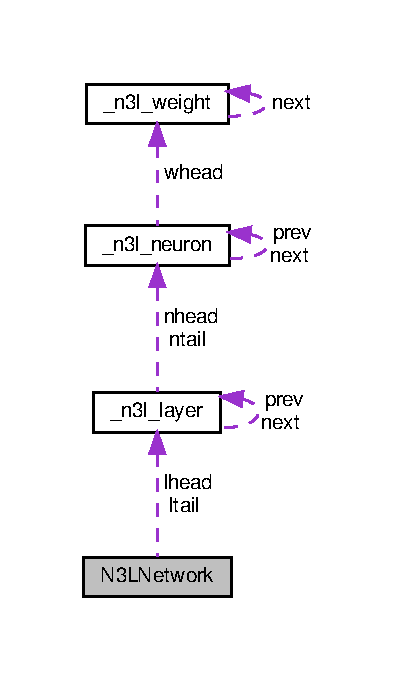
\includegraphics[width=190pt]{structN3LNetwork__coll__graph}
\end{center}
\end{figure}
\subsection*{Data Fields}
\begin{DoxyCompactItemize}
\item 
\mbox{\Hypertarget{structN3LNetwork_a45ff5bcae18502559925aba0cbd0313b}\label{structN3LNetwork_a45ff5bcae18502559925aba0cbd0313b}} 
double $\ast$ {\bfseries inputs}
\item 
\mbox{\Hypertarget{structN3LNetwork_aba0f6767a66173743840b7c9fa919daf}\label{structN3LNetwork_aba0f6767a66173743840b7c9fa919daf}} 
double $\ast$ {\bfseries targets}
\item 
\mbox{\Hypertarget{structN3LNetwork_ae7c5e2ed74786685185cf2cbb955bf51}\label{structN3LNetwork_ae7c5e2ed74786685185cf2cbb955bf51}} 
double {\bfseries learning\+\_\+rate}
\item 
\mbox{\Hypertarget{structN3LNetwork_ae77d4b7deecdc3c9590a4112689db2f8}\label{structN3LNetwork_ae77d4b7deecdc3c9590a4112689db2f8}} 
\hyperlink{struct__n3l__layer}{N3\+L\+Layer} $\ast$ {\bfseries lhead}
\item 
\mbox{\Hypertarget{structN3LNetwork_a758fd06b3dda29e064ccd4bc4d27e1c3}\label{structN3LNetwork_a758fd06b3dda29e064ccd4bc4d27e1c3}} 
\hyperlink{struct__n3l__layer}{N3\+L\+Layer} $\ast$ {\bfseries ltail}
\end{DoxyCompactItemize}


The documentation for this struct was generated from the following file\+:\begin{DoxyCompactItemize}
\item 
src/n3\+\_\+header.\+h\end{DoxyCompactItemize}

\chapter{File Documentation}
\hypertarget{n3__act_8c}{}\section{src/n3\+\_\+act.c File Reference}
\label{n3__act_8c}\index{src/n3\+\_\+act.\+c@{src/n3\+\_\+act.\+c}}


This file contains activation functions and their primitive.  


{\ttfamily \#include $<$assert.\+h$>$}\newline
{\ttfamily \#include $<$math.\+h$>$}\newline
{\ttfamily \#include \char`\"{}n3\+\_\+header.\+h\char`\"{}}\newline
Include dependency graph for n3\+\_\+act.\+c\+:\nopagebreak
\begin{figure}[H]
\begin{center}
\leavevmode
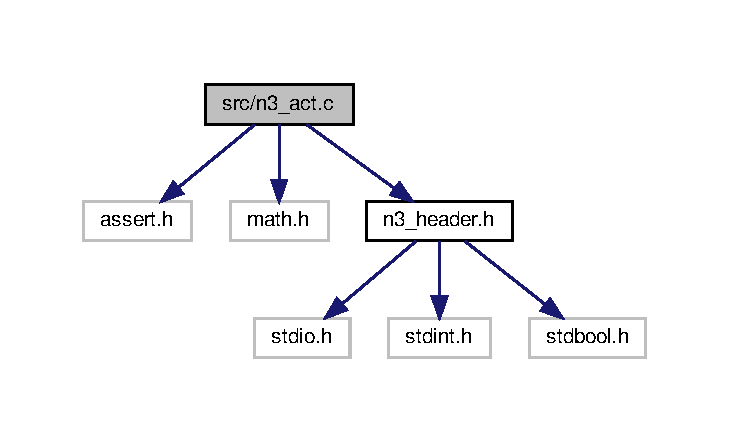
\includegraphics[width=350pt]{n3__act_8c__incl}
\end{center}
\end{figure}
\subsection*{Macros}
\begin{DoxyCompactItemize}
\item 
\#define \mbox{\hyperlink{n3__act_8c_a5347f97ed167ced1e9ffb374f218d479}{N3\+L\+\_\+\+A\+BS}}(x)~(((x) $<$ 0) ? -\/(x) \+: (x))
\begin{DoxyCompactList}\small\item\em Get the absolute value of the argument passed. \end{DoxyCompactList}\end{DoxyCompactItemize}
\subsection*{Functions}
\begin{DoxyCompactItemize}
\item 
double \mbox{\hyperlink{n3__act_8c_a8dc073371b15e2574897762b54f9326c}{n3l\+\_\+act\+\_\+none}} (double val)
\begin{DoxyCompactList}\small\item\em Doesn\textquotesingle{}t change the value passed as argument. \end{DoxyCompactList}\item 
double \mbox{\hyperlink{n3__act_8c_ad01dde283500e1fbac8d916967bfd883}{n3l\+\_\+act\+\_\+sigmoid}} (double val)
\begin{DoxyCompactList}\small\item\em Sigmoid activation function. \end{DoxyCompactList}\item 
double \mbox{\hyperlink{n3__act_8c_a4c1864b101c16c51e69a34b130fc30b6}{n3l\+\_\+act\+\_\+sigmoid\+\_\+prime}} (double val)
\begin{DoxyCompactList}\small\item\em Sigmoid activation primitive function. \end{DoxyCompactList}\item 
double \mbox{\hyperlink{n3__act_8c_aa05576ce02d1c18c0af9f042d1068c7a}{n3l\+\_\+act\+\_\+tanh}} (double val)
\begin{DoxyCompactList}\small\item\em Tanh activation function. \end{DoxyCompactList}\item 
double \mbox{\hyperlink{n3__act_8c_a24f63de53f6417037d5bebec78e08870}{n3l\+\_\+act\+\_\+tanh\+\_\+prime}} (double val)
\begin{DoxyCompactList}\small\item\em Tanh activation primitive function. \end{DoxyCompactList}\item 
double \mbox{\hyperlink{n3__act_8c_a07a8cded25f1d3b726053b50cba78eb0}{n3l\+\_\+act\+\_\+relu}} (double val)
\begin{DoxyCompactList}\small\item\em Re\+LU activation function. \end{DoxyCompactList}\item 
double \mbox{\hyperlink{n3__act_8c_ae94558725d2c300ef0879b83ee5e733a}{n3l\+\_\+act\+\_\+relu\+\_\+prime}} (double val)
\begin{DoxyCompactList}\small\item\em Re\+LU activation primitive function. \end{DoxyCompactList}\item 
double \mbox{\hyperlink{n3__act_8c_a066f6fed961da89043b1b496aa5ac6d0}{n3l\+\_\+act\+\_\+identity}} (double val)
\begin{DoxyCompactList}\small\item\em Identity activation function. \end{DoxyCompactList}\item 
double \mbox{\hyperlink{n3__act_8c_a7706b52da3c207ee1ded39ced860a138}{n3l\+\_\+act\+\_\+identity\+\_\+prime}} (double val)
\begin{DoxyCompactList}\small\item\em Identity activation primitive function. \end{DoxyCompactList}\item 
double \mbox{\hyperlink{n3__act_8c_a9e9cd6045617a4063602ccd9e94281bf}{n3l\+\_\+act\+\_\+softsign}} (double val)
\begin{DoxyCompactList}\small\item\em Soft\+Sign activation function. \end{DoxyCompactList}\item 
double \mbox{\hyperlink{n3__act_8c_aeb7c71c9bb444a3a875b7838064c8bb4}{n3l\+\_\+act\+\_\+softsign\+\_\+prime}} (double val)
\begin{DoxyCompactList}\small\item\em Soft\+Sign activation primitive function. \end{DoxyCompactList}\item 
double \mbox{\hyperlink{n3__act_8c_a2091491a8d0155701b6170c324b52eef}{n3l\+\_\+act\+\_\+leaky\+\_\+relu}} (double val)
\begin{DoxyCompactList}\small\item\em Leaky Re\+LU activation function. \end{DoxyCompactList}\item 
double \mbox{\hyperlink{n3__act_8c_a326894c0edd659426f5deaec6abe5182}{n3l\+\_\+act\+\_\+leaky\+\_\+relu\+\_\+prime}} (double val)
\begin{DoxyCompactList}\small\item\em Leaky Re\+LU activation primitive function. \end{DoxyCompactList}\item 
double \mbox{\hyperlink{n3__act_8c_ab678727eab04c73e227d0511f10da9ab}{n3l\+\_\+act\+\_\+softplus}} (double val)
\begin{DoxyCompactList}\small\item\em Soft\+Plus activation function. \end{DoxyCompactList}\item 
double \mbox{\hyperlink{n3__act_8c_a405fc712bf5abf365c90a343c664c273}{n3l\+\_\+act\+\_\+softplus\+\_\+prime}} (double val)
\begin{DoxyCompactList}\small\item\em Soft\+Plus activation primitive function. \end{DoxyCompactList}\item 
double \mbox{\hyperlink{n3__act_8c_a64fdb17c0915027691ad0b1340bdb1af}{n3l\+\_\+act\+\_\+swish}} (double val)
\begin{DoxyCompactList}\small\item\em Swish activation function. \end{DoxyCompactList}\item 
double \mbox{\hyperlink{n3__act_8c_ac0171e96a4e3c4220a4a0353e77f042b}{n3l\+\_\+act\+\_\+swish\+\_\+prime}} (double val)
\begin{DoxyCompactList}\small\item\em Swish activation primitive function. \end{DoxyCompactList}\item 
N3\+L\+Act \mbox{\hyperlink{n3__act_8c_af9034678bae2b94ebcf0d9b2ac5cfcb7}{n3l\+\_\+act}} (N3\+L\+Act\+Type type)
\begin{DoxyCompactList}\small\item\em Get the pointer to an activation function. \end{DoxyCompactList}\item 
N3\+L\+Act \mbox{\hyperlink{n3__act_8c_a9253520cb5a58edf61f04997c3161f21}{n3l\+\_\+act\+\_\+prime}} (N3\+L\+Act\+Type type)
\begin{DoxyCompactList}\small\item\em Get the pointer to an activation primitive function. \end{DoxyCompactList}\end{DoxyCompactItemize}


\subsection{Detailed Description}
This file contains activation functions and their primitive. 

\begin{DoxyAuthor}{Author}
Davide Francesco Merico 
\end{DoxyAuthor}
\begin{DoxySeeAlso}{See also}
\href{https://en.wikipedia.org/wiki/Activation_function}{\tt Wikipedia -\/ Activation Function} 
\end{DoxySeeAlso}
\begin{DoxyNote}{Note}
These functions, except for n3l\+\_\+act or n3l\+\_\+act\+\_\+prime, shouldn\textquotesingle{}t be used directly to improve compatibility with future library versions. 
\end{DoxyNote}


\subsection{Macro Definition Documentation}
\mbox{\Hypertarget{n3__act_8c_a5347f97ed167ced1e9ffb374f218d479}\label{n3__act_8c_a5347f97ed167ced1e9ffb374f218d479}} 
\index{n3\+\_\+act.\+c@{n3\+\_\+act.\+c}!N3\+L\+\_\+\+A\+BS@{N3\+L\+\_\+\+A\+BS}}
\index{N3\+L\+\_\+\+A\+BS@{N3\+L\+\_\+\+A\+BS}!n3\+\_\+act.\+c@{n3\+\_\+act.\+c}}
\subsubsection{\texorpdfstring{N3\+L\+\_\+\+A\+BS}{N3L\_ABS}}
{\footnotesize\ttfamily \#define N3\+L\+\_\+\+A\+BS(\begin{DoxyParamCaption}\item[{}]{x }\end{DoxyParamCaption})~(((x) $<$ 0) ? -\/(x) \+: (x))}



Get the absolute value of the argument passed. 


\begin{DoxyParams}{Parameters}
{\em x} & value \\
\hline
\end{DoxyParams}
\begin{DoxyReturn}{Returns}
x if x is positive, otherwise -\/x. 
\end{DoxyReturn}


\subsection{Function Documentation}
\mbox{\Hypertarget{n3__act_8c_af9034678bae2b94ebcf0d9b2ac5cfcb7}\label{n3__act_8c_af9034678bae2b94ebcf0d9b2ac5cfcb7}} 
\index{n3\+\_\+act.\+c@{n3\+\_\+act.\+c}!n3l\+\_\+act@{n3l\+\_\+act}}
\index{n3l\+\_\+act@{n3l\+\_\+act}!n3\+\_\+act.\+c@{n3\+\_\+act.\+c}}
\subsubsection{\texorpdfstring{n3l\+\_\+act()}{n3l\_act()}}
{\footnotesize\ttfamily N3\+L\+Act n3l\+\_\+act (\begin{DoxyParamCaption}\item[{N3\+L\+Act\+Type}]{type }\end{DoxyParamCaption})}



Get the pointer to an activation function. 


\begin{DoxyParams}{Parameters}
{\em type} & Activation function type. \\
\hline
\end{DoxyParams}
\begin{DoxyReturn}{Returns}
Pointer to the function chosen.
\end{DoxyReturn}
\begin{DoxySeeAlso}{See also}
\mbox{\hyperlink{n3__act_8c_a9253520cb5a58edf61f04997c3161f21}{n3l\+\_\+act\+\_\+prime}}, N3\+L\+Act, N3\+L\+Act\+Tye 
\end{DoxySeeAlso}
\mbox{\Hypertarget{n3__act_8c_a066f6fed961da89043b1b496aa5ac6d0}\label{n3__act_8c_a066f6fed961da89043b1b496aa5ac6d0}} 
\index{n3\+\_\+act.\+c@{n3\+\_\+act.\+c}!n3l\+\_\+act\+\_\+identity@{n3l\+\_\+act\+\_\+identity}}
\index{n3l\+\_\+act\+\_\+identity@{n3l\+\_\+act\+\_\+identity}!n3\+\_\+act.\+c@{n3\+\_\+act.\+c}}
\subsubsection{\texorpdfstring{n3l\+\_\+act\+\_\+identity()}{n3l\_act\_identity()}}
{\footnotesize\ttfamily double n3l\+\_\+act\+\_\+identity (\begin{DoxyParamCaption}\item[{double}]{val }\end{DoxyParamCaption})}



Identity activation function. 

\[identity(value) = value\]


\begin{DoxyParams}{Parameters}
{\em val} & input value \\
\hline
\end{DoxyParams}
\begin{DoxyReturn}{Returns}
the results from the formula above.
\end{DoxyReturn}
\begin{DoxySeeAlso}{See also}
\mbox{\hyperlink{n3__act_8c_a7706b52da3c207ee1ded39ced860a138}{n3l\+\_\+act\+\_\+identity\+\_\+prime}}, \mbox{\hyperlink{n3__act_8c_a8dc073371b15e2574897762b54f9326c}{n3l\+\_\+act\+\_\+none}}, \mbox{\hyperlink{n3__act_8c_af9034678bae2b94ebcf0d9b2ac5cfcb7}{n3l\+\_\+act}}, N3\+L\+Act, N3\+L\+Act\+Tye 
\end{DoxySeeAlso}
\mbox{\Hypertarget{n3__act_8c_a7706b52da3c207ee1ded39ced860a138}\label{n3__act_8c_a7706b52da3c207ee1ded39ced860a138}} 
\index{n3\+\_\+act.\+c@{n3\+\_\+act.\+c}!n3l\+\_\+act\+\_\+identity\+\_\+prime@{n3l\+\_\+act\+\_\+identity\+\_\+prime}}
\index{n3l\+\_\+act\+\_\+identity\+\_\+prime@{n3l\+\_\+act\+\_\+identity\+\_\+prime}!n3\+\_\+act.\+c@{n3\+\_\+act.\+c}}
\subsubsection{\texorpdfstring{n3l\+\_\+act\+\_\+identity\+\_\+prime()}{n3l\_act\_identity\_prime()}}
{\footnotesize\ttfamily double n3l\+\_\+act\+\_\+identity\+\_\+prime (\begin{DoxyParamCaption}\item[{double}]{val }\end{DoxyParamCaption})}



Identity activation primitive function. 

\[f'(value)=1\]


\begin{DoxyParams}{Parameters}
{\em val} & input value \\
\hline
\end{DoxyParams}
\begin{DoxyReturn}{Returns}
the results from the formula above.
\end{DoxyReturn}
\begin{DoxySeeAlso}{See also}
\mbox{\hyperlink{n3__act_8c_a066f6fed961da89043b1b496aa5ac6d0}{n3l\+\_\+act\+\_\+identity}}, \mbox{\hyperlink{n3__act_8c_a9253520cb5a58edf61f04997c3161f21}{n3l\+\_\+act\+\_\+prime}}, N3\+L\+Act, N3\+L\+Act\+Tye 
\end{DoxySeeAlso}
\mbox{\Hypertarget{n3__act_8c_a2091491a8d0155701b6170c324b52eef}\label{n3__act_8c_a2091491a8d0155701b6170c324b52eef}} 
\index{n3\+\_\+act.\+c@{n3\+\_\+act.\+c}!n3l\+\_\+act\+\_\+leaky\+\_\+relu@{n3l\+\_\+act\+\_\+leaky\+\_\+relu}}
\index{n3l\+\_\+act\+\_\+leaky\+\_\+relu@{n3l\+\_\+act\+\_\+leaky\+\_\+relu}!n3\+\_\+act.\+c@{n3\+\_\+act.\+c}}
\subsubsection{\texorpdfstring{n3l\+\_\+act\+\_\+leaky\+\_\+relu()}{n3l\_act\_leaky\_relu()}}
{\footnotesize\ttfamily double n3l\+\_\+act\+\_\+leaky\+\_\+relu (\begin{DoxyParamCaption}\item[{double}]{val }\end{DoxyParamCaption})}



Leaky Re\+LU activation function. 

\[leaky\_relu(value) = \begin{cases} 0.01value & \text{for } value < 0\\ value & \text{for } value \ge 0\end{cases}\]


\begin{DoxyParams}{Parameters}
{\em val} & input value \\
\hline
\end{DoxyParams}
\begin{DoxyReturn}{Returns}
the results from the formula above.
\end{DoxyReturn}
\begin{DoxySeeAlso}{See also}
\mbox{\hyperlink{n3__act_8c_a326894c0edd659426f5deaec6abe5182}{n3l\+\_\+act\+\_\+leaky\+\_\+relu\+\_\+prime}}, \mbox{\hyperlink{n3__act_8c_af9034678bae2b94ebcf0d9b2ac5cfcb7}{n3l\+\_\+act}}, N3\+L\+Act, N3\+L\+Act\+Tye 
\end{DoxySeeAlso}
\mbox{\Hypertarget{n3__act_8c_a326894c0edd659426f5deaec6abe5182}\label{n3__act_8c_a326894c0edd659426f5deaec6abe5182}} 
\index{n3\+\_\+act.\+c@{n3\+\_\+act.\+c}!n3l\+\_\+act\+\_\+leaky\+\_\+relu\+\_\+prime@{n3l\+\_\+act\+\_\+leaky\+\_\+relu\+\_\+prime}}
\index{n3l\+\_\+act\+\_\+leaky\+\_\+relu\+\_\+prime@{n3l\+\_\+act\+\_\+leaky\+\_\+relu\+\_\+prime}!n3\+\_\+act.\+c@{n3\+\_\+act.\+c}}
\subsubsection{\texorpdfstring{n3l\+\_\+act\+\_\+leaky\+\_\+relu\+\_\+prime()}{n3l\_act\_leaky\_relu\_prime()}}
{\footnotesize\ttfamily double n3l\+\_\+act\+\_\+leaky\+\_\+relu\+\_\+prime (\begin{DoxyParamCaption}\item[{double}]{val }\end{DoxyParamCaption})}



Leaky Re\+LU activation primitive function. 

\[f'(value) = \begin{cases} 0.01 & \text{for } value < 0\\ 1 & \text{for } value \ge 0\end{cases}\]


\begin{DoxyParams}{Parameters}
{\em val} & input value \\
\hline
\end{DoxyParams}
\begin{DoxyReturn}{Returns}
the results from the formula above.
\end{DoxyReturn}
\begin{DoxySeeAlso}{See also}
\mbox{\hyperlink{n3__act_8c_a2091491a8d0155701b6170c324b52eef}{n3l\+\_\+act\+\_\+leaky\+\_\+relu}}, \mbox{\hyperlink{n3__act_8c_a9253520cb5a58edf61f04997c3161f21}{n3l\+\_\+act\+\_\+prime}}, N3\+L\+Act, N3\+L\+Act\+Tye 
\end{DoxySeeAlso}
\mbox{\Hypertarget{n3__act_8c_a8dc073371b15e2574897762b54f9326c}\label{n3__act_8c_a8dc073371b15e2574897762b54f9326c}} 
\index{n3\+\_\+act.\+c@{n3\+\_\+act.\+c}!n3l\+\_\+act\+\_\+none@{n3l\+\_\+act\+\_\+none}}
\index{n3l\+\_\+act\+\_\+none@{n3l\+\_\+act\+\_\+none}!n3\+\_\+act.\+c@{n3\+\_\+act.\+c}}
\subsubsection{\texorpdfstring{n3l\+\_\+act\+\_\+none()}{n3l\_act\_none()}}
{\footnotesize\ttfamily double n3l\+\_\+act\+\_\+none (\begin{DoxyParamCaption}\item[{double}]{val }\end{DoxyParamCaption})}



Doesn\textquotesingle{}t change the value passed as argument. 

Used when no activation function is needed, by default is used for input layer\textquotesingle{}s neurons.

\[none(value) = value\]


\begin{DoxyParams}{Parameters}
{\em val} & input value \\
\hline
\end{DoxyParams}
\begin{DoxyReturn}{Returns}
the same value passed as argument.
\end{DoxyReturn}
\begin{DoxySeeAlso}{See also}
\mbox{\hyperlink{n3__act_8c_a066f6fed961da89043b1b496aa5ac6d0}{n3l\+\_\+act\+\_\+identity}}, \mbox{\hyperlink{n3__act_8c_af9034678bae2b94ebcf0d9b2ac5cfcb7}{n3l\+\_\+act}}, N3\+L\+Act, N3\+L\+Act\+Tye 
\end{DoxySeeAlso}
\mbox{\Hypertarget{n3__act_8c_a9253520cb5a58edf61f04997c3161f21}\label{n3__act_8c_a9253520cb5a58edf61f04997c3161f21}} 
\index{n3\+\_\+act.\+c@{n3\+\_\+act.\+c}!n3l\+\_\+act\+\_\+prime@{n3l\+\_\+act\+\_\+prime}}
\index{n3l\+\_\+act\+\_\+prime@{n3l\+\_\+act\+\_\+prime}!n3\+\_\+act.\+c@{n3\+\_\+act.\+c}}
\subsubsection{\texorpdfstring{n3l\+\_\+act\+\_\+prime()}{n3l\_act\_prime()}}
{\footnotesize\ttfamily N3\+L\+Act n3l\+\_\+act\+\_\+prime (\begin{DoxyParamCaption}\item[{N3\+L\+Act\+Type}]{type }\end{DoxyParamCaption})}



Get the pointer to an activation primitive function. 


\begin{DoxyParams}{Parameters}
{\em type} & Activation function type. \\
\hline
\end{DoxyParams}
\begin{DoxyReturn}{Returns}
Pointer to the function\textquotesingle{}s primitive chosen.
\end{DoxyReturn}
\begin{DoxySeeAlso}{See also}
\mbox{\hyperlink{n3__act_8c_af9034678bae2b94ebcf0d9b2ac5cfcb7}{n3l\+\_\+act}}, N3\+L\+Act, N3\+L\+Act\+Tye 
\end{DoxySeeAlso}
\mbox{\Hypertarget{n3__act_8c_a07a8cded25f1d3b726053b50cba78eb0}\label{n3__act_8c_a07a8cded25f1d3b726053b50cba78eb0}} 
\index{n3\+\_\+act.\+c@{n3\+\_\+act.\+c}!n3l\+\_\+act\+\_\+relu@{n3l\+\_\+act\+\_\+relu}}
\index{n3l\+\_\+act\+\_\+relu@{n3l\+\_\+act\+\_\+relu}!n3\+\_\+act.\+c@{n3\+\_\+act.\+c}}
\subsubsection{\texorpdfstring{n3l\+\_\+act\+\_\+relu()}{n3l\_act\_relu()}}
{\footnotesize\ttfamily double n3l\+\_\+act\+\_\+relu (\begin{DoxyParamCaption}\item[{double}]{val }\end{DoxyParamCaption})}



Re\+LU activation function. 

\[relu(value) = \begin{cases} 0 & \text{ if } value < 0 \\ value& \text{ if } value \geq 0 \end{cases}\]


\begin{DoxyParams}{Parameters}
{\em val} & input value \\
\hline
\end{DoxyParams}
\begin{DoxyReturn}{Returns}
the results from the formula above.
\end{DoxyReturn}
\begin{DoxySeeAlso}{See also}
\mbox{\hyperlink{n3__act_8c_ae94558725d2c300ef0879b83ee5e733a}{n3l\+\_\+act\+\_\+relu\+\_\+prime}}, \mbox{\hyperlink{n3__act_8c_af9034678bae2b94ebcf0d9b2ac5cfcb7}{n3l\+\_\+act}}, N3\+L\+Act, N3\+L\+Act\+Tye 
\end{DoxySeeAlso}
\mbox{\Hypertarget{n3__act_8c_ae94558725d2c300ef0879b83ee5e733a}\label{n3__act_8c_ae94558725d2c300ef0879b83ee5e733a}} 
\index{n3\+\_\+act.\+c@{n3\+\_\+act.\+c}!n3l\+\_\+act\+\_\+relu\+\_\+prime@{n3l\+\_\+act\+\_\+relu\+\_\+prime}}
\index{n3l\+\_\+act\+\_\+relu\+\_\+prime@{n3l\+\_\+act\+\_\+relu\+\_\+prime}!n3\+\_\+act.\+c@{n3\+\_\+act.\+c}}
\subsubsection{\texorpdfstring{n3l\+\_\+act\+\_\+relu\+\_\+prime()}{n3l\_act\_relu\_prime()}}
{\footnotesize\ttfamily double n3l\+\_\+act\+\_\+relu\+\_\+prime (\begin{DoxyParamCaption}\item[{double}]{val }\end{DoxyParamCaption})}



Re\+LU activation primitive function. 

\[(value)= \begin{cases} 0 & \text{ if } value < 0 \\ 1& \text{ if } value \geq 0 \end{cases}\]


\begin{DoxyParams}{Parameters}
{\em val} & input value \\
\hline
\end{DoxyParams}
\begin{DoxyReturn}{Returns}
the results from the formula above.
\end{DoxyReturn}
\begin{DoxySeeAlso}{See also}
\mbox{\hyperlink{n3__act_8c_a07a8cded25f1d3b726053b50cba78eb0}{n3l\+\_\+act\+\_\+relu}}, \mbox{\hyperlink{n3__act_8c_a9253520cb5a58edf61f04997c3161f21}{n3l\+\_\+act\+\_\+prime}}, N3\+L\+Act, N3\+L\+Act\+Tye 
\end{DoxySeeAlso}
\mbox{\Hypertarget{n3__act_8c_ad01dde283500e1fbac8d916967bfd883}\label{n3__act_8c_ad01dde283500e1fbac8d916967bfd883}} 
\index{n3\+\_\+act.\+c@{n3\+\_\+act.\+c}!n3l\+\_\+act\+\_\+sigmoid@{n3l\+\_\+act\+\_\+sigmoid}}
\index{n3l\+\_\+act\+\_\+sigmoid@{n3l\+\_\+act\+\_\+sigmoid}!n3\+\_\+act.\+c@{n3\+\_\+act.\+c}}
\subsubsection{\texorpdfstring{n3l\+\_\+act\+\_\+sigmoid()}{n3l\_act\_sigmoid()}}
{\footnotesize\ttfamily double n3l\+\_\+act\+\_\+sigmoid (\begin{DoxyParamCaption}\item[{double}]{val }\end{DoxyParamCaption})}



Sigmoid activation function. 

\[sigmoid(value) = \frac{1}{1+ e^{-value}}\]


\begin{DoxyParams}{Parameters}
{\em val} & input value \\
\hline
\end{DoxyParams}
\begin{DoxyReturn}{Returns}
the results from the formula above.
\end{DoxyReturn}
\begin{DoxySeeAlso}{See also}
\mbox{\hyperlink{n3__act_8c_a4c1864b101c16c51e69a34b130fc30b6}{n3l\+\_\+act\+\_\+sigmoid\+\_\+prime}}, \mbox{\hyperlink{n3__act_8c_af9034678bae2b94ebcf0d9b2ac5cfcb7}{n3l\+\_\+act}}, N3\+L\+Act, N3\+L\+Act\+Tye 
\end{DoxySeeAlso}
\mbox{\Hypertarget{n3__act_8c_a4c1864b101c16c51e69a34b130fc30b6}\label{n3__act_8c_a4c1864b101c16c51e69a34b130fc30b6}} 
\index{n3\+\_\+act.\+c@{n3\+\_\+act.\+c}!n3l\+\_\+act\+\_\+sigmoid\+\_\+prime@{n3l\+\_\+act\+\_\+sigmoid\+\_\+prime}}
\index{n3l\+\_\+act\+\_\+sigmoid\+\_\+prime@{n3l\+\_\+act\+\_\+sigmoid\+\_\+prime}!n3\+\_\+act.\+c@{n3\+\_\+act.\+c}}
\subsubsection{\texorpdfstring{n3l\+\_\+act\+\_\+sigmoid\+\_\+prime()}{n3l\_act\_sigmoid\_prime()}}
{\footnotesize\ttfamily double n3l\+\_\+act\+\_\+sigmoid\+\_\+prime (\begin{DoxyParamCaption}\item[{double}]{val }\end{DoxyParamCaption})}



Sigmoid activation primitive function. 

\[f'(value)= sigmoid(value) * (1 - sigmoid(value))\]


\begin{DoxyParams}{Parameters}
{\em val} & input value \\
\hline
\end{DoxyParams}
\begin{DoxyReturn}{Returns}
the results from the formula above.
\end{DoxyReturn}
\begin{DoxySeeAlso}{See also}
\mbox{\hyperlink{n3__act_8c_ad01dde283500e1fbac8d916967bfd883}{n3l\+\_\+act\+\_\+sigmoid}}, \mbox{\hyperlink{n3__act_8c_a9253520cb5a58edf61f04997c3161f21}{n3l\+\_\+act\+\_\+prime}}, N3\+L\+Act, N3\+L\+Act\+Tye 
\end{DoxySeeAlso}
\mbox{\Hypertarget{n3__act_8c_ab678727eab04c73e227d0511f10da9ab}\label{n3__act_8c_ab678727eab04c73e227d0511f10da9ab}} 
\index{n3\+\_\+act.\+c@{n3\+\_\+act.\+c}!n3l\+\_\+act\+\_\+softplus@{n3l\+\_\+act\+\_\+softplus}}
\index{n3l\+\_\+act\+\_\+softplus@{n3l\+\_\+act\+\_\+softplus}!n3\+\_\+act.\+c@{n3\+\_\+act.\+c}}
\subsubsection{\texorpdfstring{n3l\+\_\+act\+\_\+softplus()}{n3l\_act\_softplus()}}
{\footnotesize\ttfamily double n3l\+\_\+act\+\_\+softplus (\begin{DoxyParamCaption}\item[{double}]{val }\end{DoxyParamCaption})}



Soft\+Plus activation function. 

\[softplus(value) = \ln(1 + e^{value})\]


\begin{DoxyParams}{Parameters}
{\em val} & input value \\
\hline
\end{DoxyParams}
\begin{DoxyReturn}{Returns}
the results from the formula above.
\end{DoxyReturn}
\begin{DoxySeeAlso}{See also}
\mbox{\hyperlink{n3__act_8c_a405fc712bf5abf365c90a343c664c273}{n3l\+\_\+act\+\_\+softplus\+\_\+prime}}, \mbox{\hyperlink{n3__act_8c_af9034678bae2b94ebcf0d9b2ac5cfcb7}{n3l\+\_\+act}}, N3\+L\+Act, N3\+L\+Act\+Tye 
\end{DoxySeeAlso}
\mbox{\Hypertarget{n3__act_8c_a405fc712bf5abf365c90a343c664c273}\label{n3__act_8c_a405fc712bf5abf365c90a343c664c273}} 
\index{n3\+\_\+act.\+c@{n3\+\_\+act.\+c}!n3l\+\_\+act\+\_\+softplus\+\_\+prime@{n3l\+\_\+act\+\_\+softplus\+\_\+prime}}
\index{n3l\+\_\+act\+\_\+softplus\+\_\+prime@{n3l\+\_\+act\+\_\+softplus\+\_\+prime}!n3\+\_\+act.\+c@{n3\+\_\+act.\+c}}
\subsubsection{\texorpdfstring{n3l\+\_\+act\+\_\+softplus\+\_\+prime()}{n3l\_act\_softplus\_prime()}}
{\footnotesize\ttfamily double n3l\+\_\+act\+\_\+softplus\+\_\+prime (\begin{DoxyParamCaption}\item[{double}]{val }\end{DoxyParamCaption})}



Soft\+Plus activation primitive function. 

\[f'(value) = \frac{1}{1+ e^{-value}}\]


\begin{DoxyParams}{Parameters}
{\em val} & input value \\
\hline
\end{DoxyParams}
\begin{DoxyReturn}{Returns}
the results from the formula above.
\end{DoxyReturn}
\begin{DoxySeeAlso}{See also}
\mbox{\hyperlink{n3__act_8c_ab678727eab04c73e227d0511f10da9ab}{n3l\+\_\+act\+\_\+softplus}}, \mbox{\hyperlink{n3__act_8c_a9253520cb5a58edf61f04997c3161f21}{n3l\+\_\+act\+\_\+prime}}, N3\+L\+Act, N3\+L\+Act\+Tye 
\end{DoxySeeAlso}
\mbox{\Hypertarget{n3__act_8c_a9e9cd6045617a4063602ccd9e94281bf}\label{n3__act_8c_a9e9cd6045617a4063602ccd9e94281bf}} 
\index{n3\+\_\+act.\+c@{n3\+\_\+act.\+c}!n3l\+\_\+act\+\_\+softsign@{n3l\+\_\+act\+\_\+softsign}}
\index{n3l\+\_\+act\+\_\+softsign@{n3l\+\_\+act\+\_\+softsign}!n3\+\_\+act.\+c@{n3\+\_\+act.\+c}}
\subsubsection{\texorpdfstring{n3l\+\_\+act\+\_\+softsign()}{n3l\_act\_softsign()}}
{\footnotesize\ttfamily double n3l\+\_\+act\+\_\+softsign (\begin{DoxyParamCaption}\item[{double}]{val }\end{DoxyParamCaption})}



Soft\+Sign activation function. 

\[softsign(value)=\frac{value}{1+|value|}\]


\begin{DoxyParams}{Parameters}
{\em val} & input value \\
\hline
\end{DoxyParams}
\begin{DoxyReturn}{Returns}
the results from the formula above.
\end{DoxyReturn}
\begin{DoxySeeAlso}{See also}
\mbox{\hyperlink{n3__act_8c_aeb7c71c9bb444a3a875b7838064c8bb4}{n3l\+\_\+act\+\_\+softsign\+\_\+prime}}, \mbox{\hyperlink{n3__act_8c_af9034678bae2b94ebcf0d9b2ac5cfcb7}{n3l\+\_\+act}}, N3\+L\+Act, N3\+L\+Act\+Tye 
\end{DoxySeeAlso}
\mbox{\Hypertarget{n3__act_8c_aeb7c71c9bb444a3a875b7838064c8bb4}\label{n3__act_8c_aeb7c71c9bb444a3a875b7838064c8bb4}} 
\index{n3\+\_\+act.\+c@{n3\+\_\+act.\+c}!n3l\+\_\+act\+\_\+softsign\+\_\+prime@{n3l\+\_\+act\+\_\+softsign\+\_\+prime}}
\index{n3l\+\_\+act\+\_\+softsign\+\_\+prime@{n3l\+\_\+act\+\_\+softsign\+\_\+prime}!n3\+\_\+act.\+c@{n3\+\_\+act.\+c}}
\subsubsection{\texorpdfstring{n3l\+\_\+act\+\_\+softsign\+\_\+prime()}{n3l\_act\_softsign\_prime()}}
{\footnotesize\ttfamily double n3l\+\_\+act\+\_\+softsign\+\_\+prime (\begin{DoxyParamCaption}\item[{double}]{val }\end{DoxyParamCaption})}



Soft\+Sign activation primitive function. 

\[f'(value)=\frac{1}{(1+|value|)^2}\]


\begin{DoxyParams}{Parameters}
{\em val} & input value \\
\hline
\end{DoxyParams}
\begin{DoxyReturn}{Returns}
the results from the formula above.
\end{DoxyReturn}
\begin{DoxySeeAlso}{See also}
\mbox{\hyperlink{n3__act_8c_a9e9cd6045617a4063602ccd9e94281bf}{n3l\+\_\+act\+\_\+softsign}}, \mbox{\hyperlink{n3__act_8c_a9253520cb5a58edf61f04997c3161f21}{n3l\+\_\+act\+\_\+prime}}, N3\+L\+Act, N3\+L\+Act\+Tye 
\end{DoxySeeAlso}
\mbox{\Hypertarget{n3__act_8c_a64fdb17c0915027691ad0b1340bdb1af}\label{n3__act_8c_a64fdb17c0915027691ad0b1340bdb1af}} 
\index{n3\+\_\+act.\+c@{n3\+\_\+act.\+c}!n3l\+\_\+act\+\_\+swish@{n3l\+\_\+act\+\_\+swish}}
\index{n3l\+\_\+act\+\_\+swish@{n3l\+\_\+act\+\_\+swish}!n3\+\_\+act.\+c@{n3\+\_\+act.\+c}}
\subsubsection{\texorpdfstring{n3l\+\_\+act\+\_\+swish()}{n3l\_act\_swish()}}
{\footnotesize\ttfamily double n3l\+\_\+act\+\_\+swish (\begin{DoxyParamCaption}\item[{double}]{val }\end{DoxyParamCaption})}



Swish activation function. 

\[swish(value)=value * sigmoid(value)\]


\begin{DoxyParams}{Parameters}
{\em val} & input value \\
\hline
\end{DoxyParams}
\begin{DoxyReturn}{Returns}
the results from the formula above.
\end{DoxyReturn}
\begin{DoxySeeAlso}{See also}
\mbox{\hyperlink{n3__act_8c_ac0171e96a4e3c4220a4a0353e77f042b}{n3l\+\_\+act\+\_\+swish\+\_\+prime}}, \mbox{\hyperlink{n3__act_8c_af9034678bae2b94ebcf0d9b2ac5cfcb7}{n3l\+\_\+act}}, N3\+L\+Act, N3\+L\+Act\+Tye 
\end{DoxySeeAlso}
\mbox{\Hypertarget{n3__act_8c_ac0171e96a4e3c4220a4a0353e77f042b}\label{n3__act_8c_ac0171e96a4e3c4220a4a0353e77f042b}} 
\index{n3\+\_\+act.\+c@{n3\+\_\+act.\+c}!n3l\+\_\+act\+\_\+swish\+\_\+prime@{n3l\+\_\+act\+\_\+swish\+\_\+prime}}
\index{n3l\+\_\+act\+\_\+swish\+\_\+prime@{n3l\+\_\+act\+\_\+swish\+\_\+prime}!n3\+\_\+act.\+c@{n3\+\_\+act.\+c}}
\subsubsection{\texorpdfstring{n3l\+\_\+act\+\_\+swish\+\_\+prime()}{n3l\_act\_swish\_prime()}}
{\footnotesize\ttfamily double n3l\+\_\+act\+\_\+swish\+\_\+prime (\begin{DoxyParamCaption}\item[{double}]{val }\end{DoxyParamCaption})}



Swish activation primitive function. 

\[f'(value)=swish(value) + sigmoid(value) * (1 - swish(value))\]


\begin{DoxyParams}{Parameters}
{\em val} & input value \\
\hline
\end{DoxyParams}
\begin{DoxyReturn}{Returns}
the results from the formula above.
\end{DoxyReturn}
\begin{DoxySeeAlso}{See also}
\mbox{\hyperlink{n3__act_8c_a64fdb17c0915027691ad0b1340bdb1af}{n3l\+\_\+act\+\_\+swish}}, \mbox{\hyperlink{n3__act_8c_a9253520cb5a58edf61f04997c3161f21}{n3l\+\_\+act\+\_\+prime}}, N3\+L\+Act, N3\+L\+Act\+Tye 
\end{DoxySeeAlso}
\mbox{\Hypertarget{n3__act_8c_aa05576ce02d1c18c0af9f042d1068c7a}\label{n3__act_8c_aa05576ce02d1c18c0af9f042d1068c7a}} 
\index{n3\+\_\+act.\+c@{n3\+\_\+act.\+c}!n3l\+\_\+act\+\_\+tanh@{n3l\+\_\+act\+\_\+tanh}}
\index{n3l\+\_\+act\+\_\+tanh@{n3l\+\_\+act\+\_\+tanh}!n3\+\_\+act.\+c@{n3\+\_\+act.\+c}}
\subsubsection{\texorpdfstring{n3l\+\_\+act\+\_\+tanh()}{n3l\_act\_tanh()}}
{\footnotesize\ttfamily double n3l\+\_\+act\+\_\+tanh (\begin{DoxyParamCaption}\item[{double}]{val }\end{DoxyParamCaption})}



Tanh activation function. 

\[tanh(value)= \frac{e^{value}-e^{-value}}{e^{value}+e^{-value}}\]


\begin{DoxyParams}{Parameters}
{\em val} & input value \\
\hline
\end{DoxyParams}
\begin{DoxyReturn}{Returns}
the results from the formula above.
\end{DoxyReturn}
\begin{DoxySeeAlso}{See also}
\mbox{\hyperlink{n3__act_8c_a24f63de53f6417037d5bebec78e08870}{n3l\+\_\+act\+\_\+tanh\+\_\+prime}}, \mbox{\hyperlink{n3__act_8c_af9034678bae2b94ebcf0d9b2ac5cfcb7}{n3l\+\_\+act}}, N3\+L\+Act, N3\+L\+Act\+Tye 
\end{DoxySeeAlso}
\mbox{\Hypertarget{n3__act_8c_a24f63de53f6417037d5bebec78e08870}\label{n3__act_8c_a24f63de53f6417037d5bebec78e08870}} 
\index{n3\+\_\+act.\+c@{n3\+\_\+act.\+c}!n3l\+\_\+act\+\_\+tanh\+\_\+prime@{n3l\+\_\+act\+\_\+tanh\+\_\+prime}}
\index{n3l\+\_\+act\+\_\+tanh\+\_\+prime@{n3l\+\_\+act\+\_\+tanh\+\_\+prime}!n3\+\_\+act.\+c@{n3\+\_\+act.\+c}}
\subsubsection{\texorpdfstring{n3l\+\_\+act\+\_\+tanh\+\_\+prime()}{n3l\_act\_tanh\_prime()}}
{\footnotesize\ttfamily double n3l\+\_\+act\+\_\+tanh\+\_\+prime (\begin{DoxyParamCaption}\item[{double}]{val }\end{DoxyParamCaption})}



Tanh activation primitive function. 

\[f'(value) = 1 - tanh(value)^{2}\]


\begin{DoxyParams}{Parameters}
{\em val} & input value \\
\hline
\end{DoxyParams}
\begin{DoxyReturn}{Returns}
the results from the formula above.
\end{DoxyReturn}
\begin{DoxySeeAlso}{See also}
\mbox{\hyperlink{n3__act_8c_aa05576ce02d1c18c0af9f042d1068c7a}{n3l\+\_\+act\+\_\+tanh}}, \mbox{\hyperlink{n3__act_8c_a9253520cb5a58edf61f04997c3161f21}{n3l\+\_\+act\+\_\+prime}}, N3\+L\+Act, N3\+L\+Act\+Tye 
\end{DoxySeeAlso}

%--- End generated contents ---

% Index
\backmatter
\newpage
\phantomsection
\clearemptydoublepage
\addcontentsline{toc}{chapter}{Index}
\printindex

\end{document}
